\chapter{Introduction}

\section{Context}

\par
%Identify the problem
Programming is like building something with primitive blocks and it can be a very difficult task if we have to program every aspect of the application without some “blocks” already built for us to use.
That’s why in the programming world there is a whole panoply of free and commercial libraries with APIs that provide a huge quantity of functions for the programmer to use.

\par
In computer graphics, there are many libraries that provide functionalities to render images based in different techniques.
Ray tracing is a technique for rendering an image by tracing the path of light through pixels in an image plane and simulating the effects of its interactions with virtual objects.
This technique is capable of producing a very high degree of visual realism but at a great computational cost.

\par
Since nowadays we have more and more mobile systems whose computational power increases every year, the need for more libraries to help the programmers develop applications for these systems is increasing too.
However, there are not many options to choose from for developing a renderer based on ray tracing.
That’s why this dissertation focuses on assessing and providing a ray tracer library for mobile systems.

\par
%To delimit the problem
It is important to mention that this dissertation is not focused on rendering techniques other than ray tracing.
It is not focused in assess different integrators (numerical solutions to the rendering equation) and / or assess different approaches in ray tracing like Packet Traversal.
It is also not focused on assess different quasi random numbers generators neither assess the performance of different computer systems.

\par
These rendering algorithms based in ray tracing are very useful because they allow rendering photo-realistic images with a degree of realism much better than the graphics cards allow by default through rasterization.
As previously stated, the computing power in mobile devices processors has been increasing and this may allow a mobile device with a mid-range processor to run these algorithms in a useful time.

\begin{figure}[H]
\centering
\caption{Illustration of the most common mobile devices - tablet and smartphone (\cite{JournalDuNet}).}
\label{Illustration of the most common mobile devices - tablet and smartphone}
\includegraphics[width=10cm,height=10cm,keepaspectratio,scale=1.0]{Mobile_devices.jpg}
\end{figure}

\section{Motivation}

\par
Among other factors, the productivity of a programmer depends on what libraries he can have access to.
But, there are almost no rendering libraries based in ray tracing available today for mobile systems like Android, iOS, Windows 10 Mobile, BlackBerry 10, Tizen, Sailfish OS, Symbian and Ubuntu Touch.
And it is likely that these systems already have enough processing power to render images with fairly complex scenes in an acceptable time by using algorithms based in ray tracing.

\par
It is also important to note that there is not much documentation about the advantages and limitations of executing different rendering algorithms in these devices.

\par
Last but not least, it is important to mention that of all the operating systems available for mobile devices, the one chosen for the ray tracing library was Android.
Because nowadays it is the operating system with the most market share.
More than 85\% of the mobile devices use Android, and only 14\% of these devices use iOS which is the second most used operating system in these devices.
And, besides that, it allows to be executed on a variety of different devices: smart phones, tablet computers, smart TVs, smart watches and even laptop / desktop computers.

\begin{figure}[H]
	\centering
	\caption{Illustration of a variety of mobile devices compatible with Android (\cite{AndroidDevices}).}
	\label{Illustration of a variety of mobile devices compatible with Android}
	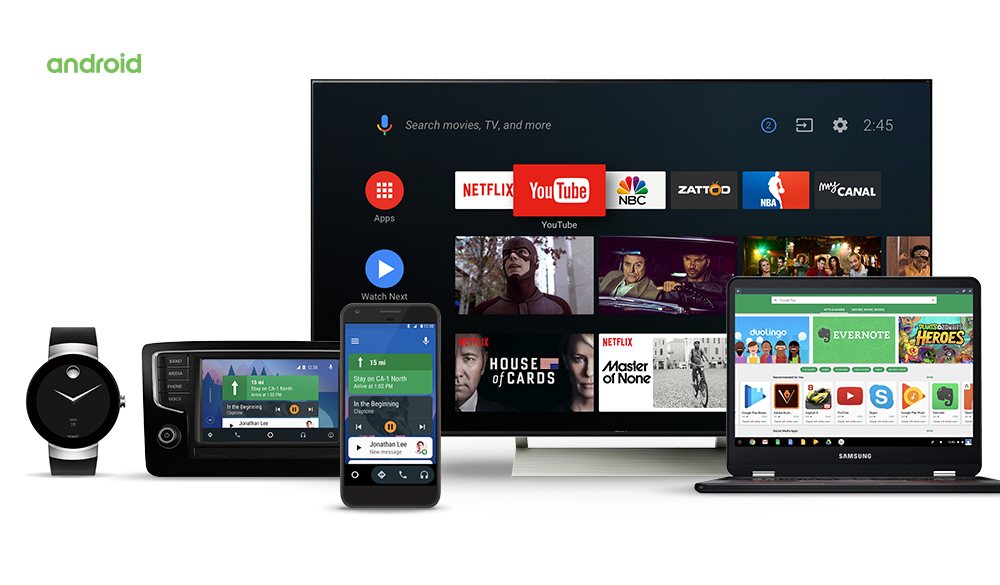
\includegraphics[width=10cm,height=10cm,keepaspectratio,scale=1.0]{Android_devices.png}
\end{figure}


\section{Goals}

\par
The main goal of this dissertation is to assess and demonstrate the advantages of running rendering algorithms in mobile devices.

\par
It is also intended to promote and facilitate the development of applications for mobile systems that use ray tracing techniques, with special emphasis on rendering applications.
To do this, will be developed a library that supports the fundamental operations of a ray tracing engine.
This library will allow the agile development of diverse applications, by using components that invoke the functionality of the library itself.

\par
Additionally, it is intended to supply rendering components at a higher abstraction level, like the camera, scene and the integrator that facilitates further the development of applications.

\par
Finally, it is important to do a demonstration of the rendering application with some interface layer to let the user assess the performance of several functionalities provided by the library.

\section{Document Structure}

\par
This dissertation is organized in five chapters: Introduction, State of the Art, Software Architecture, Demonstration: Global Illumination and Conclusion \& Future work.

\par
The first chapter describes the context and motivation behind this work, as well as its goals.
Its main purpose is to identify the problem at hand and set up goals that should be accomplished.

\par
The second chapter introduces the main concepts of ray tracing and compares different implementations of ray tracers already available in the world wide web.
The reason behind this comparison is to show how many ray tracers are already available to mobile devices and highlight the differences between the features they have.
It also provides some information about the processors of today that helps realize their ability to execute computationally demanding algorithms like ray tracing.

\par
The third chapter explains the proposed approach and explains each module developed in the library and in the rendering components.
This chapter ends with an explanation of some Android specifics, such as the user interface by characterizing its work flow and mentioning some of the challenges overcame during the development of the application.

\par
The fourth chapter summarizes the key results obtained by executing different algorithms with different number of threads and different acceleration structures.
And it will also contain a small comparison between the developed application and the Android CPU Raytracer (\cite{Android_CPU_Raytracer}).

\par
Finally, the fifth chapter ends this dissertation with the conclusions that can be withdrawn from this work and proposes some future work.